\subsubsection{User experience design and testing}
Usability is a \emph{`quality attribute that assesses how easy interfaces are to use'} (\cite{usabilitycomponentsnielsen}). The best way to assess the usability of an interface is to conduct usability testing.\\
Also referred to as \emph{user testing} is a popular UX research methodology used to uncover problems in the user interface design of an application and learn about the target user's preferences (\cite{usertestingdefinition}).\\

\noindent There are 3 core elements to user testing: \textbf{the facilitator}, \textbf{the participant} and \textbf{the tasks}. The facilitator administers the tasks to the participant, observes their behaviour and listens to their feedback.\\

\noindent Our approach is as follows:
%user evaluation process
\begin{figure}[h!]
    \centering
    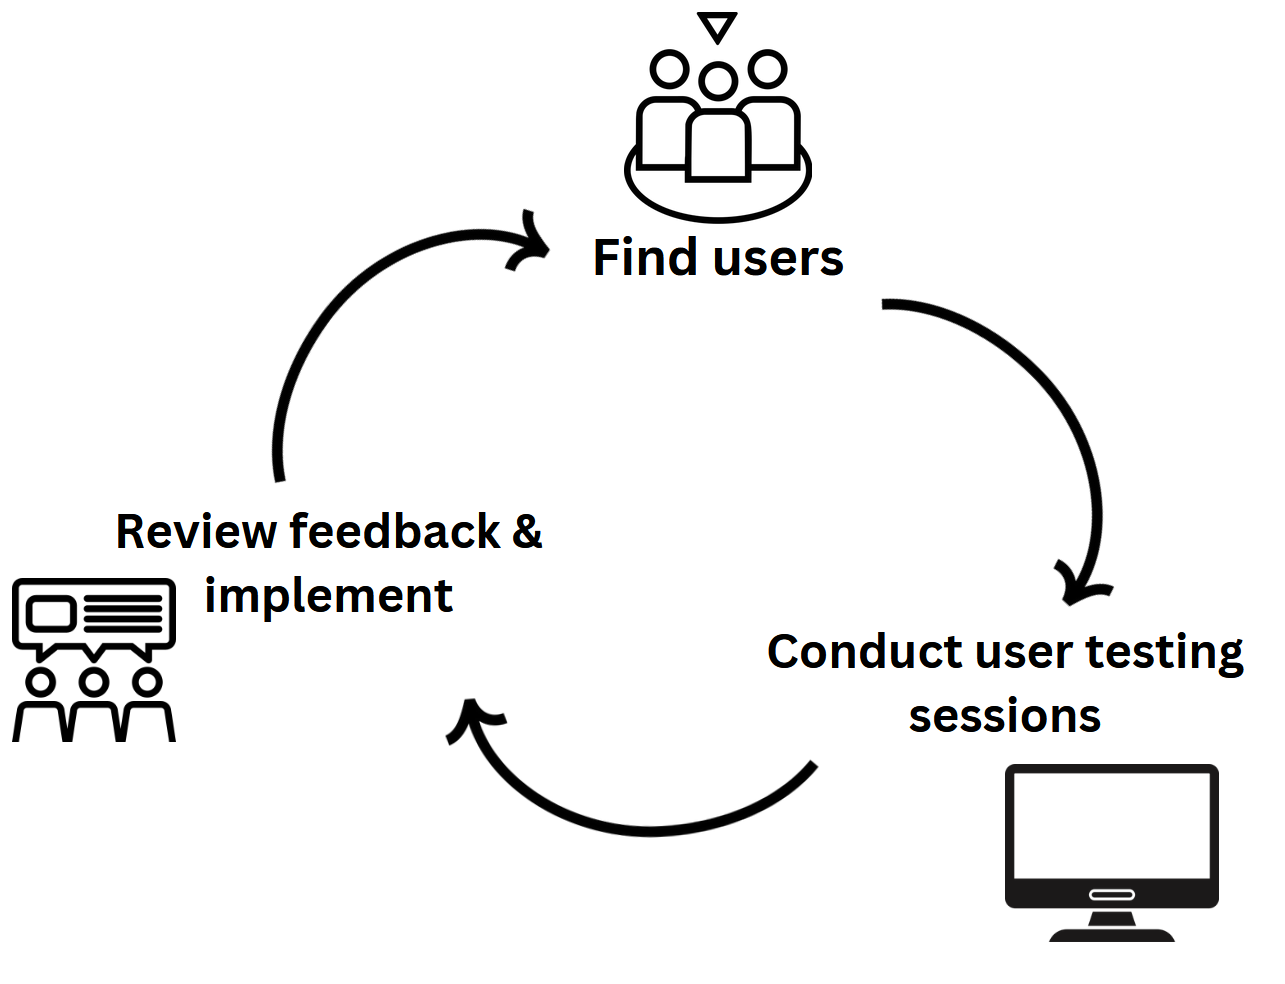
\includegraphics[width=0.6\textwidth]{images/user-eval-process.png}
    \caption{User Evaluation Process}
\end{figure}\\
Firstly, we round up users from the market research survey who left their contact and seek out others through social media channels. Next, we conduct online user testing sessions to discuss Magpie, explore the features and gather feedback. We then synthesize the notes taken during the sessions and review what new features to implement, what items to change or remove. Lastly, we go over the process again in order to continue improving Magpie's workflow and interface.\\
We interviewed 11 users in total. Some have decided to remain anonymous, therefore have been labelled as \emph{Anonymous n°}, while others will be referred to by their name. \\ They have been divided into the following categories: 6 general users, 3 targeted users, 1 UI/UX expert and 1 accessibility expert.\\
\emph{General users} are defined as those who use Magpie casually for personal interests.\\ \emph{Targeted users} are defined as those who use Magpie as a tool for their work.

\noindent Both controlled \& uncontrolled approaches were used for the sessions.\\
The controlled sessions were based around a strict list of tasks the user would complete and used metrics such as time taken, difficulty and task success rate.\\
The uncontrolled sessions let the users freely roam the application while we observed their behaviour interacting with each element and initiate discussion to obtain feedback on features to improve.\\

\noindent A table with a list of general tasks is used to quantitatively evaluate each feature the user interacted with. Metrics measured are task difficulty and task success rate. The list of general tasks increased as the test sessions went on because new features were being added iteratively.\\
The difficulty of the task is related to its status and how much time a user spent on it. The status of a task can either be `complete', `pass', or `fail' where:
\begin{itemize}
    \item \emph{complete} is attributed when the user completes the task on their own
    \item \emph{pass} is attributed when the user was able to complete the task but with our help
    \item \emph{fail} is attributed when the user was not able to complete the task even with our help
\end{itemize}
Lastly, a short satisfaction survey is administered at the end of each session quantify user experience and provide a baseline for improvements. User behaviour is also observed during the session to complement these quantitative metrics.\\
%figure for satisfaction survey
\begin{figure}[h!]
    \centering
    \fbox{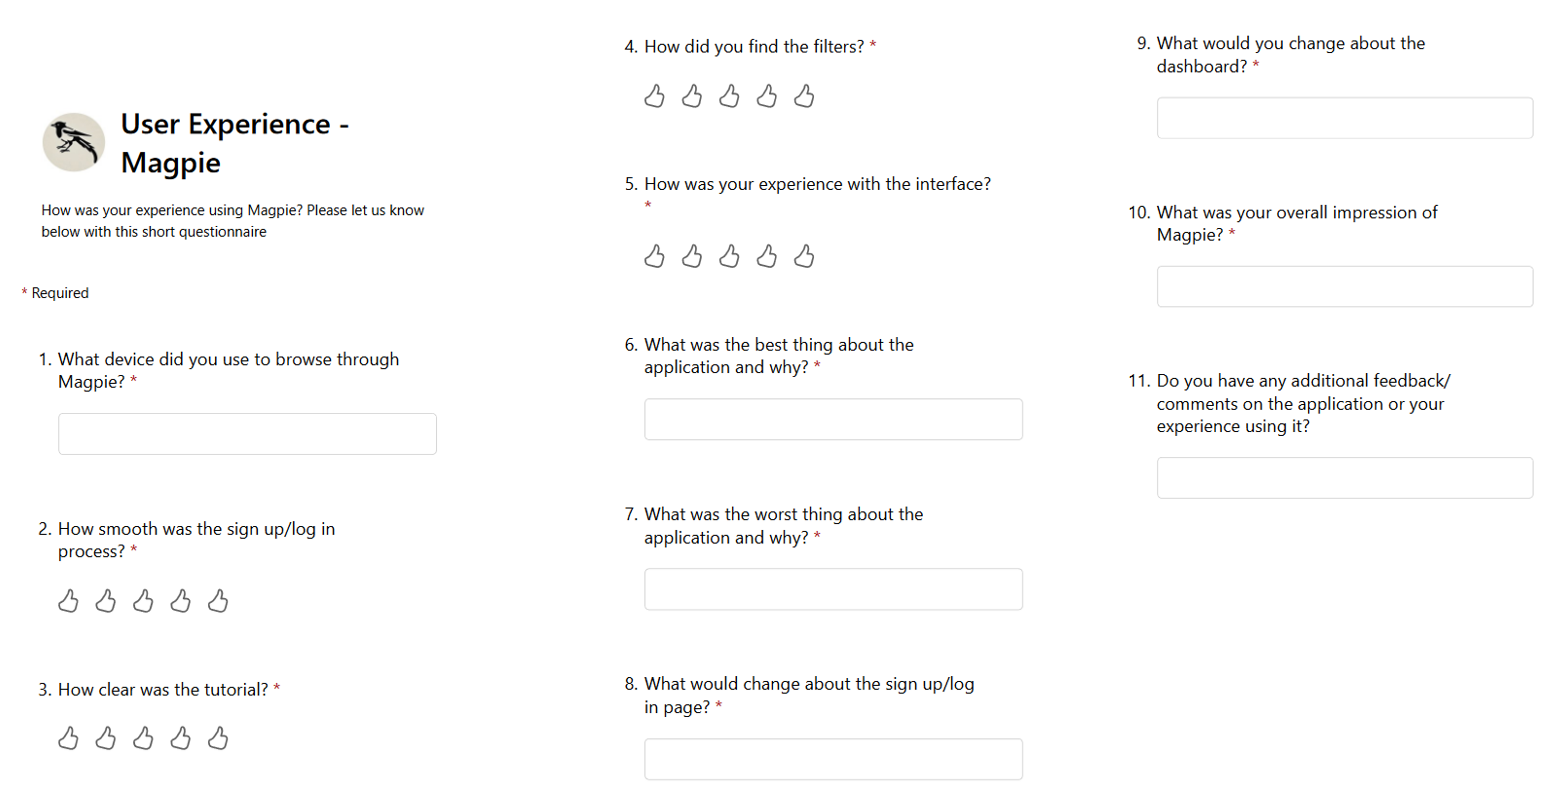
\includegraphics[width=0.8\textwidth]{images/user-satisfaction-survey.png}}
    \caption{User Evaluation - Satisfaction survey questions}
\end{figure}\\
The evaluation of Magpie has been divided into the following sections:
\begin{enumerate}
    \item General users test sessions
    \item Targeted users test sessions
    \item UX/UI expert review
    \item Accessibility expert review
\end{enumerate}
